\documentclass[]{article}
\usepackage[T1]{fontenc}

\usepackage{graphicx}
\usepackage{parskip}
\usepackage[]{hyperref}
\usepackage[french]{babel}

\author{Erwan LEMATTRE, Yannis CHUPIN}
\title{Rapport mi-projet\\Fairness pour l'IA}

\begin{document}
    \maketitle
    \newpage
    \tableofcontents
    \newpage

    \section{Introduction}
    Ce projet a pour objectif d'analyser les accidents de la circulation routière afin de pouvoir dire 
    à partir des données d'un véhicule accidenté si l'accident est mortel ou non.
    Les données sont des données libres mises à disposition par le \textit{Ministère de l'intérieur et des 
    Outre-Mer}. Le jeu de donnée correspond aux accidents de 2005 à 2022 en France. Nous allons dans une première 
    partie analyser ces données afin d'extraire les informations utiles à l'apprentissage et de pouvoir repérer 
    d'éventuelles sources de biais pour notre modèle.
    
    Vous pouvez retrouver le code sur le GitHub du projet. Le fichier \texttt{main.ipynb} contient 
    le code principale que nous allons suivre tout au long de ce rapport. Le fichier \texttt{utils.py} 
    contient toutes les fonctions auxilières que nous utilisons dans le fichier principale.

    \section{Découverte du jeu de données}
    \subsection{La base de données}
    La base de données est composée de plusieurs tables: \textit{usagers}, \textit{vehicules}, \textit{lieux} et 
    \textit{caracteristiques}. Nous avons joint ces quatres parties pour obtenir un dataframe contenant une 
    cinquantaine de colonnes. 
    Ci-dessous une rapide présentation des différentes données disponibles.

    \begin{center}
        \begin{tabular}{ |c|c| }
            \hline
            \textbf{Attribut} & \textbf{Description} \\
            \hline
            \textit{Num\_Acc} & Numéro d'identifiant de l'accident \\
            \textit{jour mois} & Jour de l'accident, mois de l'accident \\
            \textit{an} & Numéro d'identifiant de l'accident. \\
            \textit{hrmn} & Numéro d'identifiant de l'accident. \\
            \textit{lum} & Numéro d'identifiant de l'accident. \\
            \textit{dep} & Numéro d'identifiant de l'accident. \\
            \textit{com} & Numéro d'identifiant de l'accident. \\
            \textit{agg} & Numéro d'identifiant de l'accident. \\
            \textit{int} & Numéro d'identifiant de l'accident. \\
            \textit{atm} & Numéro d'identifiant de l'accident. \\
            \textit{col} & Numéro d'identifiant de l'accident. \\
            \textit{adr} & Numéro d'identifiant de l'accident. \\
            \textit{lat} & Numéro d'identifiant de l'accident. \\
            \textit{long} & Numéro d'identifiant de l'accident. \\
            \textit{catr} & Numéro d'identifiant de l'accident. \\        
            \hline
        \end{tabular}
    \end{center}

    \subsection{Répartition des données}
    Afin de pouvoir conserver les données utiles pour l'apprentissage nous avons analysé la répartition des 
    différentes données dans notre dataframe.
    Nous avons ainsi pu faire différentes observations. 
    \\
    Voici quelques-unes d'entre elles qui nous sont ensuite
    utiles pour la préparation des données.
    \subsubsection{Catégories de véhicule}
    La base de données nous donne beaucoup de catégories différentes. Nous avons cependant pu remarquer 
    que la majorité des véhicules sont dans seulement 5 catégories.
    \begin{figure}[ht]
        \centering
        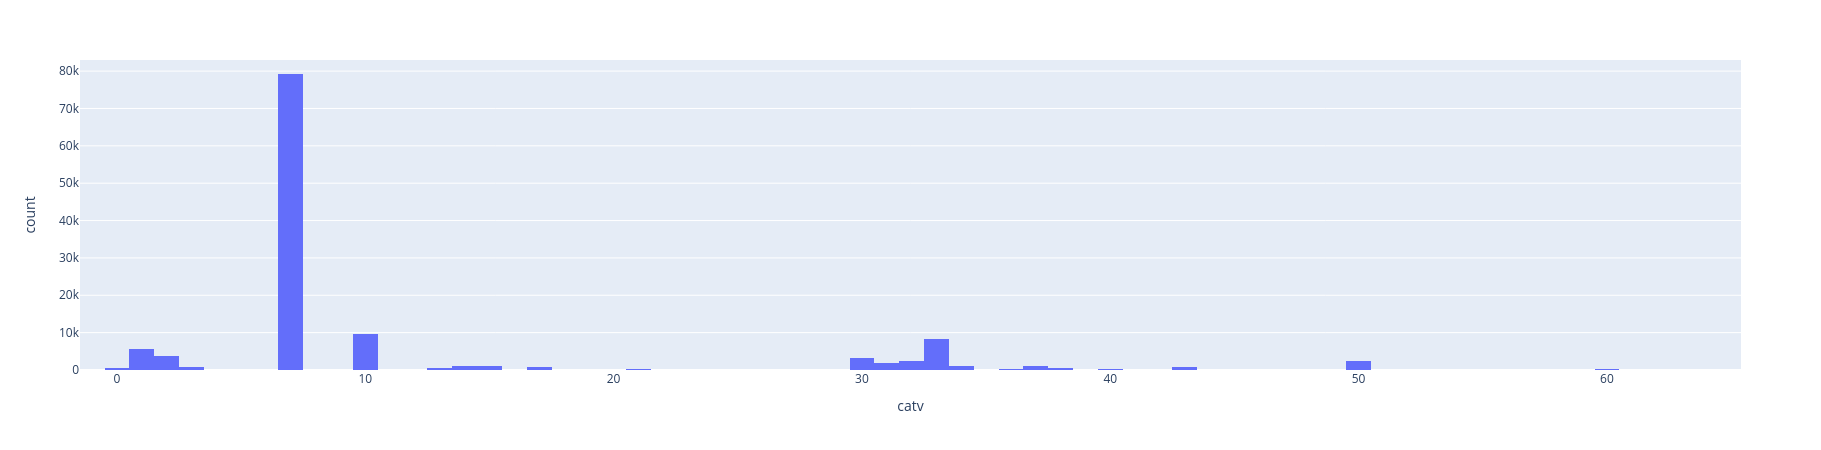
\includegraphics[width=12cm]{./img/catv1.png}
        \caption{Répartition des catégories de véhicules}
    \end{figure}

    \subsubsection{Gravité de l'accident}
    En affichant l'effectif d'accidents mortels nous avons pu remarquer qu'ils ne représentent qu'une 
    infime partie des accidents. Le peu de données sur ces accidents ne nous permet pas l'apprentissage 
    d'un modèle. C'est la raison pour laquelle nous avons décidé de nous intéresser non pas à la mortalité 
    à l'échelle d'une personne mais plutôt à l'échelle d'un accident. Nous nous mettons pour cela au niveau d'un 
    véhiule car cela nous permet de conserver plus d'informations (à l'échelle d'un accident on aurait 
    dû enlever trop d'informations pour conserver seulement les attributs plus généraux à l'accident).

    \begin{figure}[ht]
        \centering
        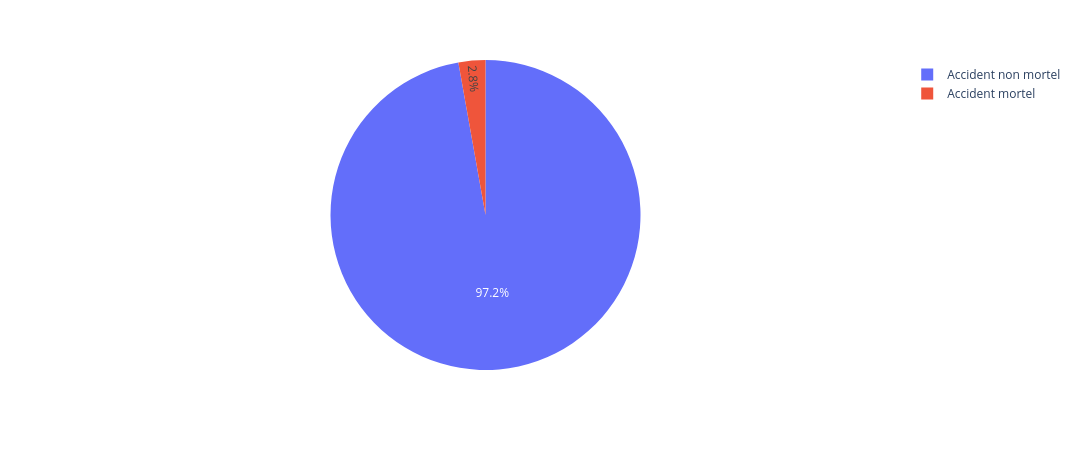
\includegraphics[width=12cm]{./img/grav1.png}
        \caption{Proportion d'accidents mortels}
    \end{figure}

    \section{Préparation des données}
    À partir des observations précédentes, nous avons supprimé les attributs moins intéressant pour l'apprentissage 
    et nous avons modifié certains attributs afin d'en extraire les informations intéressantes.
    \\
    Les attributs supprimés sont: \textit{voie}, \textit{v1}, \textit{v2}, \textit{pr}, \textit{pr1}, \textit{lartpc},
     \textit{larrout}, \textit{num\_veh}, \textit{occutc}, \textit{adr}, \textit{senc}, \textit{etatp}, \textit{actp}, 
     \textit{manv}, \textit{jour}, \textit{com}, \textit{hrmn}, \textit{motor}, \textit{place}, \textit{vosp}, \textit{locp}.
    \\\\
    Nous avons effectué les modifications suivantes:
    \begin{itemize}
        \item Création d'un attribut \textit{mortal} qui vaut 1 si le véhicule est impliqué dans un accident mortel, 0 sinon.
        \item À partir de l'attribut \textit{sexe} nous avons créé un attribut \textit{sexe\_conducteur} qui garde seulement 
                le sexe du conducteur du véhicule.
        \item Création d'un attribut \textit{piéton} qui vaut 1 si un piéton est impliqué dans l'accident, sinon 0.
        \item Nous avons utilisé l'année de naissance et l'année de l'accident pour récupérer l'âge du conducteur.
        \item L'attribut \textit{vma} a été découpé en 4 catégories de vitesse.
        \item Pour les attributs \textit{catv} et \textit{vatr} nous avons gardé les valeurs le plus représentées dans la base de données.
    \end{itemize}
    \vspace{0.5cm}
    Nous avons également reduit les valeurs de certains attributs. Par exemple pour des attributs 
    avec des valeurs telles que \textit{Non-renseigné}, \textit{Autre} \dots \, Nous avons regroupé 
    ces valeurs en une seule valeur. L'objectif était ici de simplifier en réduisant les catégories 
    mais également d'améliorer les performances de notre modèle.

    \section{Analyse des données}
    Une fois nos données préparées, nous avons pu les visualiser. Nous allons montrer dans les 
    deux prochaines parties les observations intéressantes que nous avons pu faire lors de 
    l'analyse de notre dataset.

    \subsection{Analyse univarié des données}
    \subsubsection{Les accidents mortels}
    Une donnée intéressante à observer est la proportion de véhicules impliqués dans un accident 
    mortel. C'est en effet la valeur que nous voulons prédire.

    \begin{figure}[ht]
        \centering
        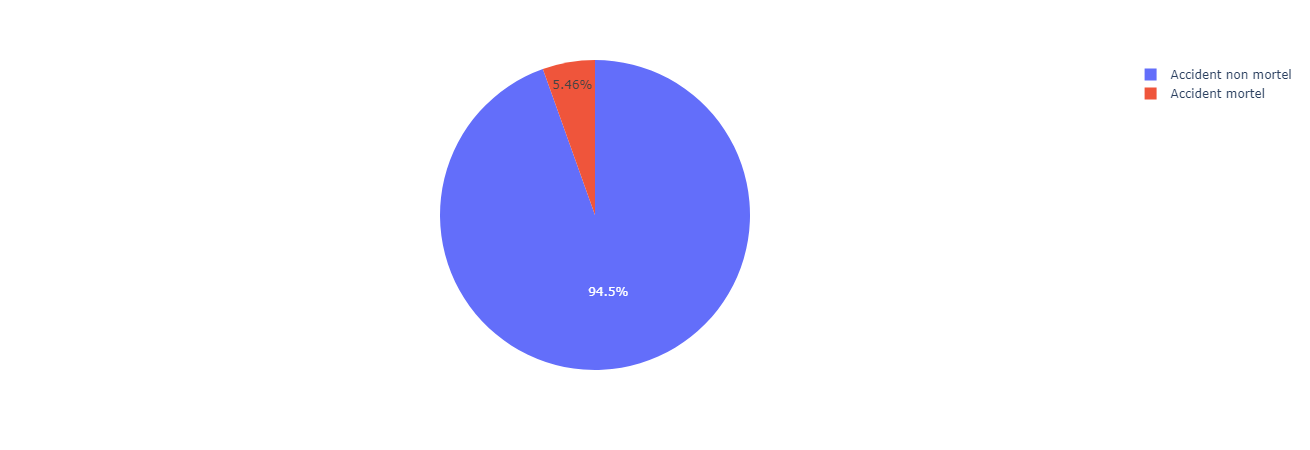
\includegraphics[width=10cm]{./img/grav2.png}
        \caption{Proportion des véhicules impliqués dans un accident mortel}
        \label{fig:fig_acc_mortel}
    \end{figure}

    Nous pouvons remarquer sur la figure \ref{fig:fig_acc_mortel} que le fait de s'intéresser 
    aux véhcules impliqués dans un accident mortel et non plus aux personnes victimes permet 
    de doubler le pourcentage. Même si cette proportion reste faible, cela va nous permettre 
    d'avoir plus de données dans la catégorie mortel lors de l'apprentissage et par conséquent 
    d'avoir un meilleur modèle.

    \subsubsection{Les piétons}
    Nous nous sommes ensuite intéressé aux accidents dans lesquels un piéton est impliqué. 
    La figure \ref{fig:fig_acc_pieton} nous montre qu'un peu moins de 10\% des accidents impliquent 
    un piéton.

    \begin{figure}[ht]
        \centering
        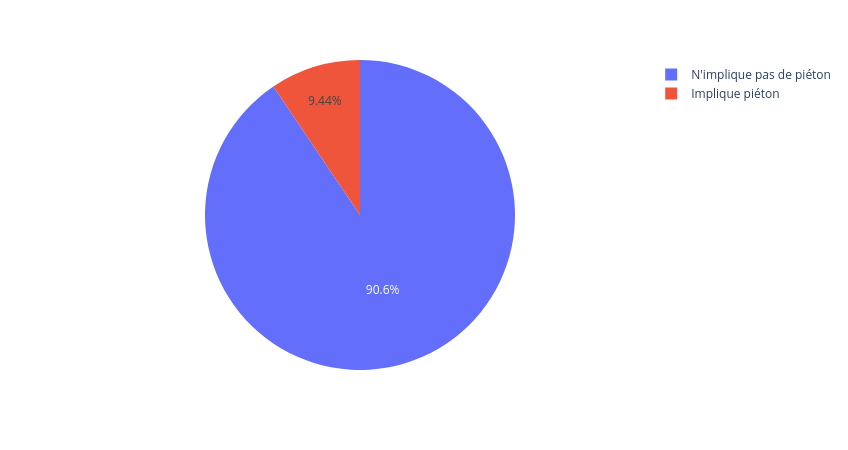
\includegraphics[width=10cm]{./img/pieton.png}
        \caption{Proportion des accidents avec piéton}
        \label{fig:fig_acc_pieton}
    \end{figure}

    \subsubsection{L'âge}
    Nous pouvons visualiser l'âge des conducteurs via une boîte à moustache. La figure \ref{fig:fig_age} nous 
    montre la répartition de l'âge des conducteurs. Lors du prétraitement des données, les valeurs aberrantes 
    ont été enlevée. On retrouve donc logiquement des âges contenus entre 0 et 100 ans. L'âge médian des 
    conducteurs est 33 ans avec le premier quatile à 21 et le troisième quatile à 49 ans. Même si on peut 
    imaginer que des valeurs sont fausse (il y a des conducteurs de moins de 16 ans), les valeurs sont tout de 
    même assez cohérentes par rapport à ce que l'on pourrait imaginer de la répartition de l'âge des conducteurs.

    \begin{figure}[ht]
        \centering
        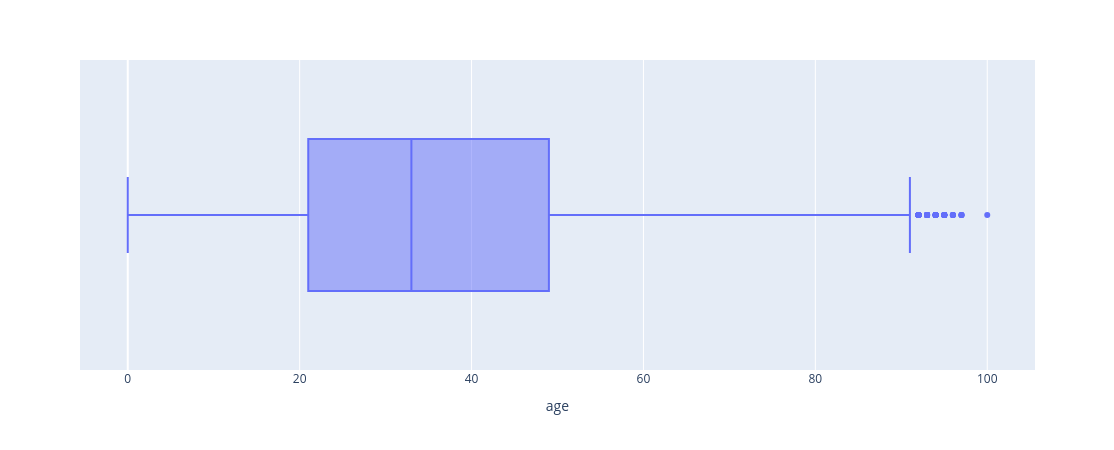
\includegraphics[width=12cm]{./img/age.png}
        \caption{Âge des conducteurs}
        \label{fig:fig_age}
    \end{figure}

    \subsubsection{Le genre des conducteurs}
    Le genre des conducteurs est assez intéressant à analyser. Sur la figure \ref{fig:fig_genre} nous pouvons 
    remarquer différence importante entre le nombre de femme au volant (indice 0) et le nombre d'hommes au volant 
    (indice 1). Cette différence pourrait être une source de biais pour notre modèle. En effet le fait qu'il y ait 
    beaucoup plus de données d'accident avec des hommes ne signifie pas qu'il y a plus de chance d'avoir un accident 
    si on est un homme. Cela signifie peut-être que la proportion d'homme au volant est plus élévée et donc qu'il 
    y a plus d'accident avec un homme au volant car il y a plus d'homme au volant. Le risque ici est que notre 
    modèle associe une homme à un accident mortel car il y a beaucoup plus d'accidents mortels avec un homme au 
    volant.

    \begin{figure}[ht]
        \centering
        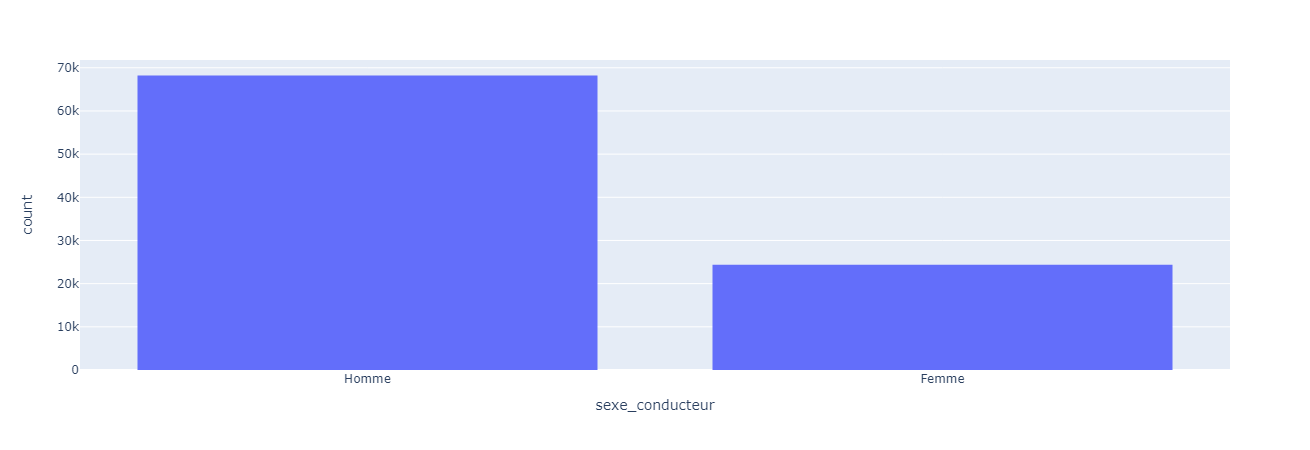
\includegraphics[width=12cm]{./img/sexe.png}
        \caption{Genre des conducteurs}
        \label{fig:fig_genre}
    \end{figure}

    \subsubsection{Le type de collision}
    La figure \ref{fig:fig_col} montre la répartition des différents types de collisions dans notre dataset. On peut 
    remarquer que tous les types de collisions sont plutôt bien représentés dans notre dataset. C'est un attribut qui 
    pourra être assez intéressant pour l'apprentissage.

    \begin{figure}[ht]
        \centering
        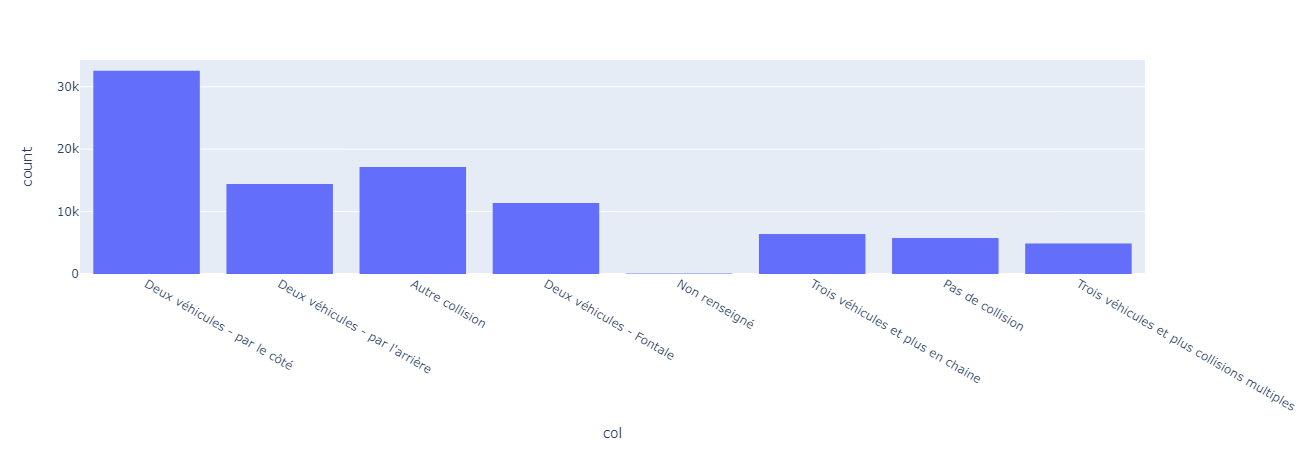
\includegraphics[width=12cm]{./img/col.png}
        \caption{Les types de collision}
        \label{fig:fig_col}
    \end{figure}

    \subsection{Analyse bivariée des données}

    \section{Apprentissage}
    \subsection{One Hot Encoding}
    Une grande partie des attributs sont des attributs numériques mais sont tout de même des attributs catégoriels.
    C'est pourquoi nous avons dû catégoriser manuellement les attributs.
    Le One Hot Encoding est ensuite effectué via le pipeline.

    \section{Audit du modèle}



\end{document}